
%(BEGIN_QUESTION)
% Copyright 2008, Tony R. Kuphaldt, released under the Creative Commons Attribution License (v 1.0)
% This means you may do almost anything with this work of mine, so long as you give me proper credit

{\it Load lines} are useful tools for analyzing transistor amplifier circuits, but they may be applied to other types of circuits as well.  Here, we will explore the application of load lines to a simple diode-resistor circuit.

The diode's characteristic curve is already plotted on the following graph, based on Shockley's diode equation shown below:

$$I_D = I_S (e^{qV_D \over NkT} - 1)$$

\noindent
Where,

$I_D =$ Current through the PN junction, in amps

$I_S =$ PN junction saturation current, in amps (typically 1 picoamp)

$e =$ Euler's number $\approx$ 2.718281828

$q =$ Electron unit charge, $1.6 \times 10^{-19}$ coulombs

$V_D =$ Voltage across the PN junction, in volts

$N =$ Nonideality coefficient, or emission coefficient (typically between 1 and 2)

$k =$ Boltzmann's constant, $1.38 \times 10^{-23}$ joules per kelvin

$T =$ Junction temperature, in degrees kelvin

$$\includegraphics[width=15.5cm]{i03223x01.eps}$$

Your task is to plot the load line for the circuit on the same graph, explaining the significance of the two plots' intersection.

\vskip 20pt \vbox{\hrule \hbox{\strut \vrule{} {\bf Suggestions for Socratic discussion} \vrule} \hrule}

\begin{itemize}
\item{} Explain why the use of a load line greatly simplifies the determination of circuit current in such a diode-resistor circuit.
\item{} Suppose the resistor value were increased from 2.5 k$\Omega$ to 10 k$\Omega$.  What difference would this make in the load line plot, and in the intersection point between the two plots?
\end{itemize}

\underbar{file i03223}
%(END_QUESTION)





%(BEGIN_ANSWER)

The two lines intersect at a current of approximately 1.72 mA:

$$\includegraphics[width=15.5cm]{i03223x03.eps}$$

%(END_ANSWER)





%(BEGIN_NOTES)

While this approach to circuit analysis may seem silly -- using load lines to calculate the current in a diode-resistor circuit -- it demonstrates the principle of load lines in a context that should be obvious to students at this point in their study.  Discuss with your students how the load line is obtained for this circuit, and why it is straight while the diode's characteristic curve is not.  

Also, discuss the significance of the two line intersecting.  Mathematically, what does the intersection of two graphs mean?  What do the coordinate values of the intersection point represent in a system of simultaneous functions?  How does this principle relate to an electronic circuit?

%INDEX% Electronics review: load lines
%INDEX% Final Control Elements, valve: characterization

%(END_NOTES)


